%%%% fs-run-time-experiments   Experiments

\label {fs-experiments-section}

\begin{figure}[htbp]
  \centering
  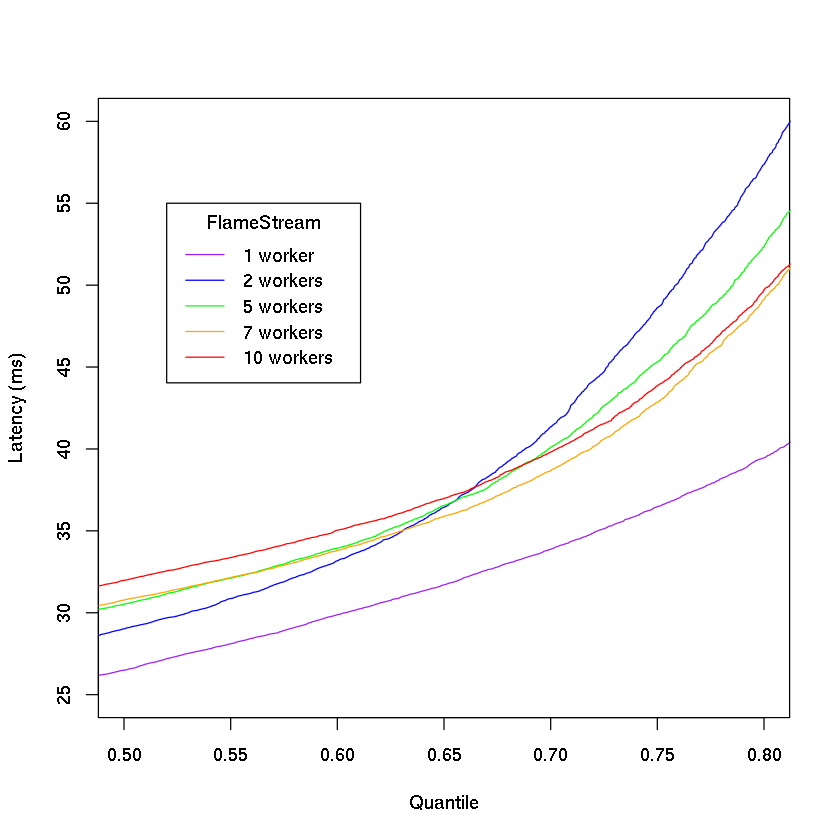
\includegraphics[width=0.48\textwidth]{pics/fs-index-median}
  \caption{FlameStream median latencies}
  \label {fs-index-median}
\end{figure}

\begin{figure}[htbp]
  \centering
  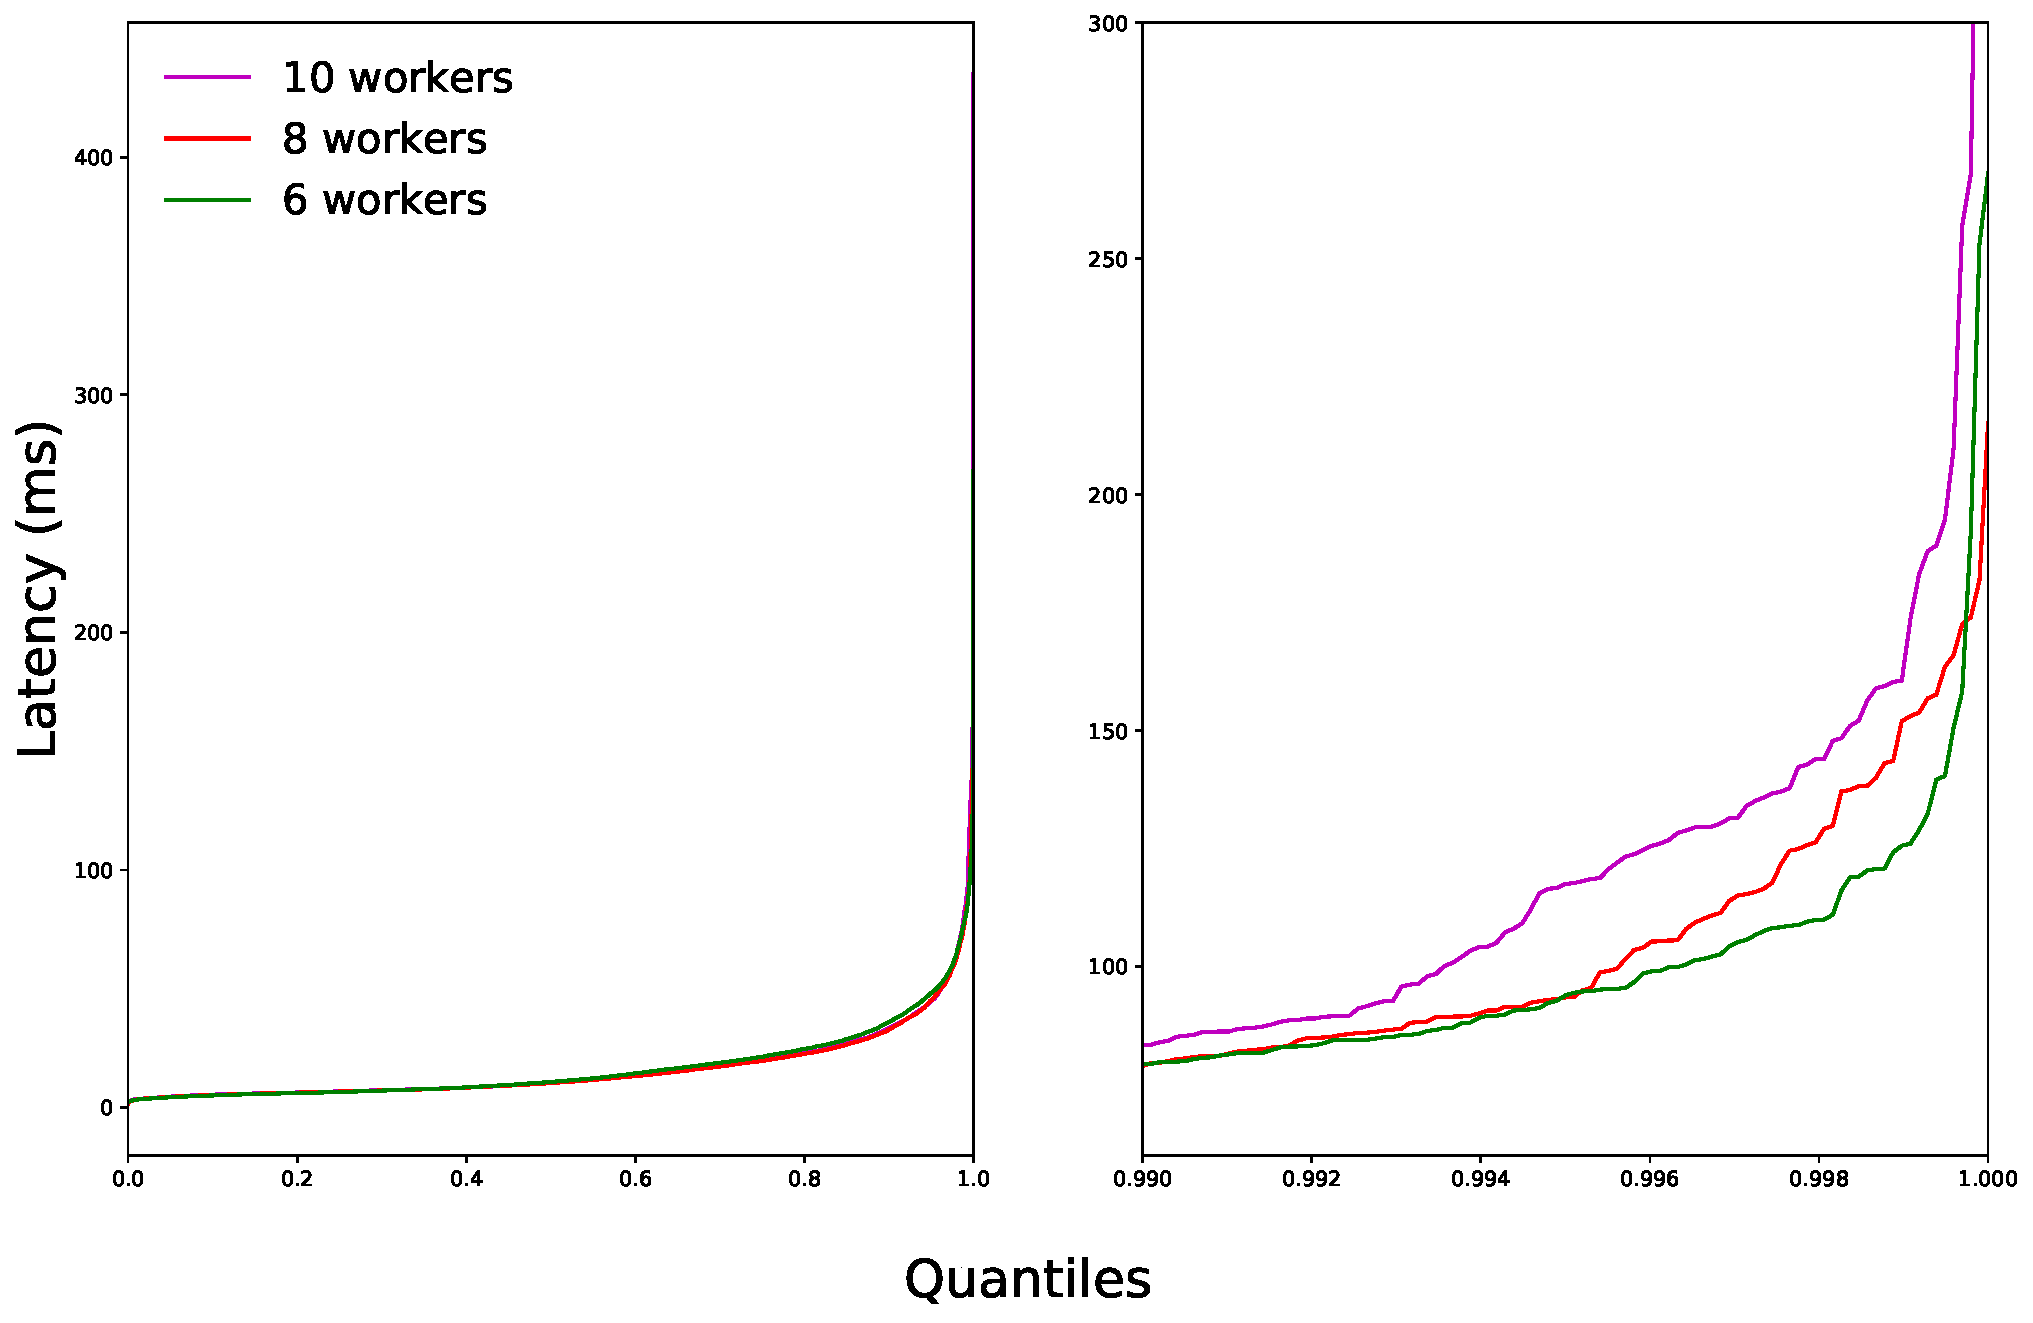
\includegraphics[width=0.48\textwidth]{pics/fs-index-quantiles}
  \caption{FlameStream tail latencies}
  \label {fs-index-quantiles}
\end{figure}

\begin{figure}[htbp]
  \centering
  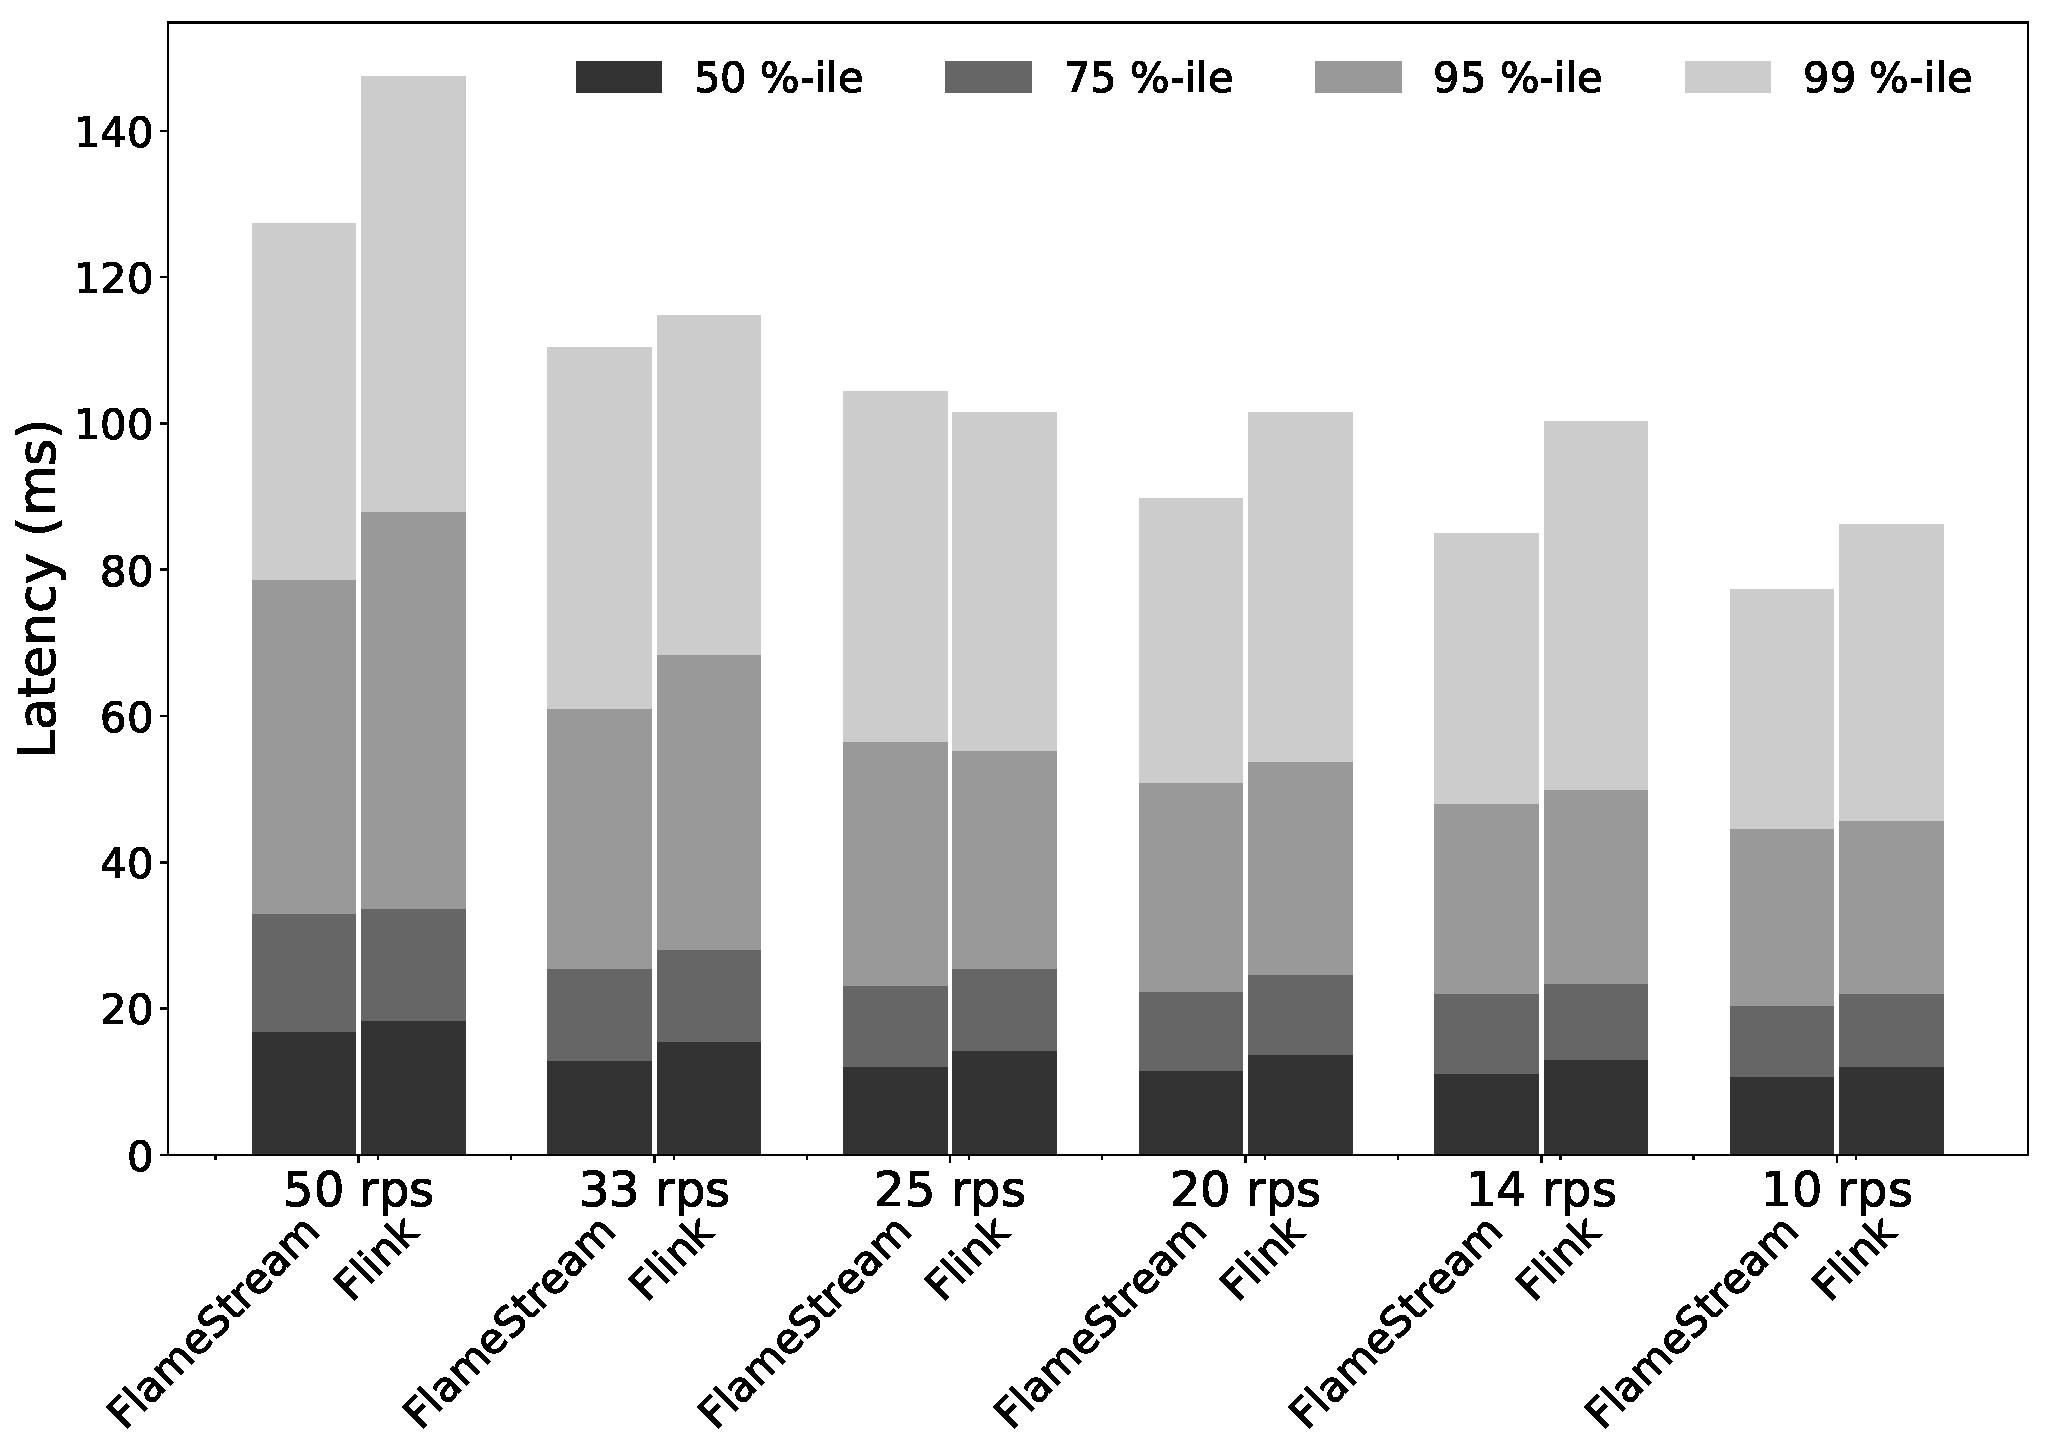
\includegraphics[width=0.48\textwidth]{pics/comp-index-quantiles}
  \caption{Latency distribution comparison}
  \label {comp-index-quantiles}
\end{figure}

The performance of Flame Stream is compared with the  performance of Flink both running on 1, 2, 3, 5 and 10 computers with data set size of 1/3, 2/3, and 1 of the whole data set  (describe the data set here).

The latency and overall processing time is measured. 
~\ref{fs-index-median}
~\ref{fs-index-quantiles}
~\ref{comp-index-quantiles}

More details on computers and operating environment are needed here.

Put results, preferable charts but tables are also good, here.

The results of experiments clearly show that we are in certain sense good.  (Please be more specific here.)

